\documentclass[10pt]{article}
\usepackage[utf8]{inputenc}
\usepackage[T1]{fontenc}
\usepackage{amsmath}
\usepackage{amsfonts}
\usepackage{amssymb}
\usepackage[version=4]{mhchem}
\usepackage{stmaryrd}
\usepackage{graphicx}
\usepackage[export]{adjustbox}
\graphicspath{ {./images/} }
\usepackage{caption}

\DeclareUnicodeCharacter{25A1}{\ifmmode\square\else{$\square$}\fi}

\begin{document}
\captionsetup{singlelinecheck=false}
\section*{Handout 29}
\section*{Optical Transitions in Solids, Optical Gain, and Semiconductor Lasers}
In this lecture you will learn:

\begin{itemize}
  \item Electron-photon Hamiltonian in solids
  \item Optical transition matrix elements
  \item Optical absorption coefficients
  \item Stimulated absorption and stimulated emission
  \item Optical gain in semiconductors
  \item Semiconductor heterostructure lasers
\end{itemize}

ECE 407 - Spring 2009 - Farhan Rana - Cornell University

\section*{Interactions Between Light and Solids}
The basic interactions between light and solids cover a wide variety of topics that can include:

\begin{itemize}
  \item Interband electronic transitions in solids
  \item Intraband electronic transitions and intersubband electronic transitions
  \item Plasmons and plasmon-polaritons
  \item Surface plasmons
  \item Excitons and exciton-polaritons
  \item Phonon and phonon-polaritons
  \item Nonlinear optics\\
-Quantum optics
  \item Optical spintronics
\end{itemize}

\section*{Fermi's Golden Rule: A Review}
Consider a Hamiltonian with the following eigenstates and eigenenergies:

$$
\hat{H}_{0}\left|\psi_{m}\right\rangle=E_{m}\left|\psi_{m}\right\rangle \quad\{m=\text { integer }
$$

Now suppose a time dependent externally applied potential is added to the Hamiltonian:

$$
\hat{H}=\hat{H}_{o}+\hat{V}_{\uparrow} e^{-i \omega t}+\hat{V}_{\downarrow} e^{i \omega t}
$$

Suppose at time $\boldsymbol{t}=\mathbf{0}$ an electron was in some initial state $\boldsymbol{k}:|\boldsymbol{\psi}(\boldsymbol{t}=\mathbf{0})\rangle=\left|\boldsymbol{\psi}_{\boldsymbol{p}}\right\rangle$\\
Fermi's golden rule tells that the rate at which the electron absorbs energy $\hbar \omega$ from the time-dependent potential and makes a transition to some higher energy level is given by:

$$
\left.W_{\uparrow}(p)=\frac{2 \pi}{\hbar} \sum_{m}\left|\left\langle\psi_{m}\right| \hat{V}_{\uparrow}\right| \psi_{p}\right\rangle\left.\right|^{2} \delta\left(E_{m}-E_{p}-\hbar \omega\right)
$$

\begin{center}
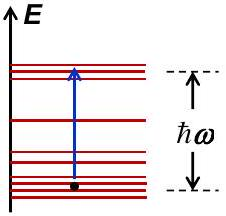
\includegraphics[max width=\textwidth, alt={}]{d3f49174-c405-454e-8341-a4302bd8c868-02_216_226_760_1375}
\end{center}

The rate at which the electron gives away energy $\hbar \omega$ to the time-dependent potential and makes a transition to some lower energy level is given by:

$$
\left.W_{\downarrow}(p)=\frac{2 \pi}{\hbar} \sum_{m}\left|\left\langle\psi_{m}\right| \hat{V}_{\downarrow}\right| \psi_{p}\right\rangle\left.\right|^{2} \delta\left(E_{m}-E_{p}+\hbar \omega\right)
$$

\begin{center}
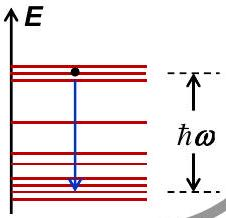
\includegraphics[max width=\textwidth, alt={}]{d3f49174-c405-454e-8341-a4302bd8c868-02_218_226_992_1375}
\end{center}

ECE 407 - Spring 2009 - Farhan Rana - Cornell University

\section*{Optical Transitions in Solids: Energy and Momentum Conservation}
For an electron to absorb energy from a photon energy conservation implies:\\
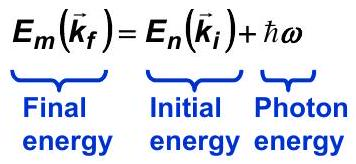
\includegraphics[max width=\textwidth, alt={}, center]{d3f49174-c405-454e-8341-a4302bd8c868-02_164_356_1695_678}

Momentum conservation implies:

$$
\underbrace{\hbar \overrightarrow{\boldsymbol{k}}_{\boldsymbol{f}}}_{\substack{\text { Final } \\ \text { momentum }}}=\underbrace{\hbar \overrightarrow{\boldsymbol{q}}}_{\substack{\text { Initial } \\ \text { momentum } \\ \hbar \overrightarrow{\boldsymbol{k}}_{i}}}
$$

\begin{center}
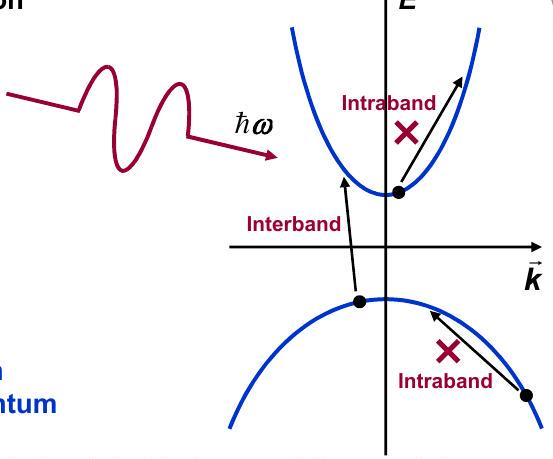
\includegraphics[max width=\textwidth, alt={}]{d3f49174-c405-454e-8341-a4302bd8c868-02_459_553_1632_1104}
\end{center}

Note that the momentum conservation principle is stated in terms of the crystal momentum of the electrons. This principle will be derived later.

Intraband photonic transitions are not possible:\\
For parabolic bands, it can be shown that intraband optical transitions cannot satisfy both energy and momentum conservation and are therefore not possible

\section*{Electromagnetic Wave Basics}
Consider an electromagnetic wave passing through a solid with electric field given by:

$$
\vec{E}(\vec{r}, t)=-\hat{n} E_{0} \sin (\vec{q} \cdot \vec{r}-\omega t)
$$

The vector potential associated with the field is:

$$
\begin{aligned}
\vec{E}(\vec{r}, t)=-\frac{\partial \vec{A}(\vec{r}, t)}{\partial t} \Rightarrow \vec{A}(\vec{r}, t) & =\hat{n} \frac{E_{0}}{\omega} \cos (\vec{q} \cdot \vec{r}-\omega t) \\
& =\hat{n} A_{0} \cos (\vec{q} \cdot \vec{r}-\omega t)
\end{aligned}
$$

The divergence of the field is zero:\\
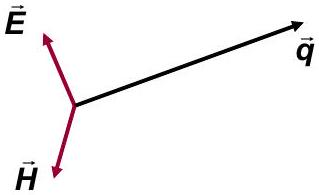
\includegraphics[max width=\textwidth, alt={}, center]{d3f49174-c405-454e-8341-a4302bd8c868-03_195_319_603_1316}

$$
\nabla \cdot \vec{E}(\vec{r}, t)=\nabla \cdot \vec{A}(\vec{r}, t)=0
$$

The power per unit area or the Intensity of the field is given by the Poynting vector:

$$
\vec{I}=\langle\vec{S}(\vec{r}, t)\rangle=\langle\vec{E}(\vec{r}, t) \times \vec{H}(\vec{r}, t)\rangle=\hat{q} \frac{E_{o}^{2}}{2 \eta}=\hat{q} \frac{\omega^{2} A_{o}^{2}}{2 \eta} \quad\left\{\eta=\sqrt{\frac{\mu_{o}}{\varepsilon}}=\frac{\eta_{\mathrm{o}}}{n}\right.
$$

The photon flux per unit area is:

$$
\boldsymbol{F}=\frac{|\overrightarrow{\boldsymbol{I}}|}{\hbar \omega}=\frac{\omega A_{o}^{2}}{2 \eta \hbar}
$$

ECE 407 - Spring 2009 - Farhan Rana - Cornell University

\section*{Electron-Photon Hamiltonian in Solids}
Consider electrons in a solid. The eigenstates (Bloch functions) and eigenenergies satisfy:

$$
\hat{H}_{0}\left|\psi_{n, \vec{k}}\right\rangle=E_{n}(\vec{k})\left|\psi_{n, \vec{k}}\right\rangle
$$

where:

$$
\hat{H}_{0}=\frac{\hat{\vec{P}} \cdot \hat{\vec{P}}}{2 m}+V_{\text {lattice }}(\hat{\vec{r}})
$$

In the presence of E\&M fields the Hamiltonian is:

$$
\begin{aligned}
\hat{H} & =\frac{[\hat{\vec{P}}+e \vec{A}(\hat{\vec{r}}, t)]^{2}}{\mathbf{2 m}}+V_{\text {lattice }}(\hat{\vec{r}}) \quad\left\{\vec{A}(\vec{r}, t)=\hat{n} A_{o} \cos (\vec{q} \cdot \vec{r}-\omega t)\right. \\
& =\frac{\hat{\vec{P}} \cdot \hat{\vec{P}}}{\mathbf{2 m}}+V_{\text {lattice }}(\hat{\vec{r}})+\frac{\mathbf{e}}{\mathbf{2 m}} \hat{\vec{P}} \cdot \vec{A}(\hat{\vec{r}}, t)+\frac{\mathbf{e}}{\mathbf{2 m}} \vec{A}(\hat{\vec{r}}, t) \cdot \hat{\vec{P}}+\frac{\mathbf{e}^{2}}{\mathbf{2 m}} \vec{A}(\hat{\vec{r}}, t) \cdot \vec{A}(\hat{\vec{r}}, t) \\
& \approx \hat{H}_{o}+\frac{\mathbf{e}}{\mathbf{2 m}} \hat{\vec{P}} \cdot \vec{A}(\hat{\vec{r}}, t)+\frac{\mathbf{e}}{\mathbf{2 m}} \vec{A}(\hat{\vec{r}}, t) \cdot \hat{\vec{P}} \\
& =\hat{H}_{o}+\frac{\mathbf{e}}{m} \vec{A}(\hat{\vec{r}}, t) \cdot \hat{\vec{P}} \longrightarrow \text { Assume small } \\
& =\hat{H}_{o}+\frac{\mathbf{e}_{o}\left[\mathbf{e}^{i \vec{q}} \cdot \hat{\vec{r}}-i \omega t+\mathbf{e}^{-i \vec{q}} \cdot \hat{\vec{r}}+i \omega t\right]}{\mathbf{2 m}} \hat{\boldsymbol{n}} \cdot \hat{\vec{P}}
\end{aligned}
$$

\section*{Optical Interband Transitions in Solids}
$$
\begin{gathered}
\hat{H}_{0}\left|\psi_{n, \vec{k}}\right\rangle=E_{n}(\vec{k})\left|\psi_{n, \vec{k}}\right\rangle \\
\hat{H}=\hat{H}_{0}+\frac{e A_{o}\left[e^{i \vec{q} \cdot \hat{\vec{r}}-i \omega t}+e^{-i \vec{q} \cdot \hat{\vec{r}}+i \omega t}\right]}{\mathbf{2 m}} \hat{\vec{P}} \cdot \hat{n}
\end{gathered}
$$

Comparison with:

$$
\hat{H}=\hat{H}_{o}+\hat{V}_{\uparrow} e^{-i \omega t}+\hat{V}_{\downarrow} e^{i \omega t}
$$

gives:

$$
\hat{V}_{\uparrow}=\frac{e A_{0} e^{i \vec{q} \cdot \hat{\vec{r}}}}{2 m} \hat{\vec{P}} \cdot \hat{n} \quad \hat{V}_{\downarrow}=\frac{e A_{0} e^{-i \vec{q} \cdot \hat{\vec{r}}}}{2 m} \hat{\vec{P}} \cdot \hat{n}
$$

Suppose at time $\boldsymbol{t}=\mathbf{0}$ the electron was sitting in the valence band with crystal momentum $\boldsymbol{k}_{\boldsymbol{i}}$ :

$$
|\psi(\boldsymbol{t}=\mathbf{0})\rangle=\left|\psi_{\boldsymbol{v}, \vec{k}_{i}}\right\rangle
$$

\begin{center}
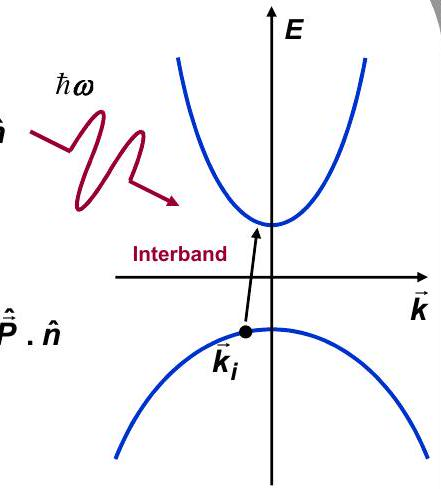
\includegraphics[max width=\textwidth, alt={}]{d3f49174-c405-454e-8341-a4302bd8c868-04_489_441_416_1218}
\end{center}

The transition rate to states in the conduction band is given by the Fermi's golden rule:

$$
\left.W_{\uparrow}\left(\vec{k}_{i}\right)=\frac{2 \pi}{\hbar} \sum_{\vec{k}_{f}}\left|\left\langle\psi_{c, \vec{k}_{f}}\right| \hat{V}_{\uparrow}\right| \psi_{v, \vec{k}_{i}}\right\rangle\left.\right|^{2} \delta\left(E_{c}\left(\vec{k}_{f}\right)-E_{v}\left(\vec{k}_{i}\right)-\hbar \omega\right)
$$

The summation is over all possible final states in the conduction band that have the same spin as the initial state. Energy conservation is enforced by the delta function.

ECE 407 - Spring 2009 - Farhan Rana - Cornell University

\section*{Optical Matrix Element}
$$
\begin{aligned}
& W_{\uparrow}\left(\vec{k}_{i}\right)=\frac{\mathbf{2} \pi}{\hbar} \sum_{\vec{k}_{f}}\left\langle\left\langle\psi_{c, \vec{k}_{f}}\right| \hat{V}_{\uparrow} \mid \psi_{v, \vec{k}_{i}}\right\rangle^{2} \delta\left(E_{c}\left(\vec{k}_{f}\right)-E_{v}\left(\vec{k}_{i}\right)-\hbar \omega\right) \\
& \quad=\frac{\mathbf{2} \pi}{\hbar}\left(\frac{\mathbf{e} A_{o}}{\mathbf{2} m}\right)^{\mathbf{2}} \sum_{\vec{k}_{f}}\left\langle\left\langle\psi_{c, \vec{k}_{f}}\right| \mathbf{e}^{i \vec{q} \cdot \hat{\vec{r}} \hat{\vec{P}} \cdot \hat{n}\left|\psi_{v, \vec{k}_{i}}\right\rangle^{2} \delta\left(E_{c}\left(\vec{k}_{f}\right)-E_{v}\left(\vec{k}_{i}\right)-\hbar \omega\right)}\right.
\end{aligned}
$$

Now consider the matrix element:

$$
\begin{aligned}
& \left\langle\psi_{c, \vec{k}_{f}}\right| e^{i \vec{q} \cdot \hat{\vec{r}} \hat{\vec{P}} \cdot \hat{n}\left|\psi_{v, \vec{k}_{i}}\right\rangle} \\
& =\int d^{3} \vec{r} \psi_{c, \vec{k}_{f}}^{*}(\vec{r}) \quad e^{i \vec{q} \cdot \vec{r}} \hat{\vec{P}} \cdot \hat{n} \quad \psi_{v, \vec{k}_{i}}(\vec{r}) \\
& =\int d^{3} \vec{r} \mathrm{e}^{-i \vec{k}_{f} \cdot \vec{r}_{u} u_{c, \vec{k}_{f}}(\vec{r})} \quad \mathrm{e}^{i \vec{q} \cdot \vec{r}} \hat{\vec{P}} \cdot \hat{n} \quad \mathrm{e}^{i \vec{k}_{i} \cdot \vec{r}} u_{v, \vec{k}_{i}}(\vec{r}) \\
& =\int d^{3} \vec{r} \mathrm{e}^{-i \vec{k}_{f} \cdot \vec{r}} u_{c, \vec{k}_{f}}^{*}(\vec{r}) \\
& =\int \mathrm{e}^{i \vec{q} \cdot \vec{r}} \mathrm{e}^{i \vec{k}_{i} \cdot \vec{r}}\left(\hat{\vec{P}}+t \vec{k}_{i}\right) \cdot \hat{n} \quad u_{v, \vec{k}_{i}}(\vec{r}) \\
& =\int d^{3} \vec{r} \mathrm{e}^{-i \vec{k}_{f} \cdot \vec{r}} u_{c, \vec{k}_{f}}^{*}(\vec{r}) \quad \mathrm{e}^{i \vec{q} \cdot \vec{r}} \mathrm{e}^{i \vec{k}_{i} \cdot \vec{r}} \hat{\vec{P}} \cdot \hat{n} \quad u_{v, \vec{k}_{i}}(\vec{r})
\end{aligned}
$$

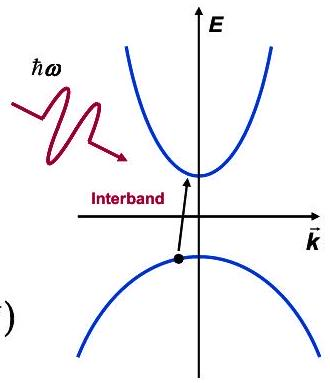
\includegraphics[max width=\textwidth, alt={}, center]{d3f49174-c405-454e-8341-a4302bd8c868-04_383_330_1811_1323}\\
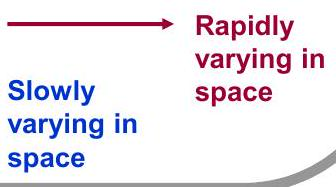
\includegraphics[max width=\textwidth, alt={}, center]{d3f49174-c405-454e-8341-a4302bd8c868-04_187_336_2230_1274}

ECE 407 - Spring 2009 - Farhan Rana - Cornell University

$$
\begin{aligned}
& \left\langle\boldsymbol{\psi}_{\boldsymbol{c}, \overrightarrow{\boldsymbol{k}}_{\boldsymbol{f}}}\right| \mathbf{e}^{i \overline{\boldsymbol{q}} \cdot \hat{\dot{r}} \hat{\overline{\boldsymbol{P}}} \cdot \hat{\boldsymbol{n}}}\left|\boldsymbol{\psi}_{\boldsymbol{v}, \overrightarrow{\boldsymbol{k}}_{\boldsymbol{i}}}\right\rangle \\
& =\int d^{3} \vec{r} e^{-i \vec{k}_{f} \cdot \vec{r} u^{*}}{ }_{c, \vec{k}_{f}}(\vec{r}) \quad e^{i \vec{q} \cdot \vec{r}} e^{i \vec{k}_{i} \cdot \vec{r}} \hat{\vec{P}} \cdot \hat{n} \quad u_{v, \vec{k}_{i}}(\vec{r}) \\
& =\sum_{\vec{R}_{j}} e^{i\left(\vec{k}_{i}+\vec{q}-\vec{k}_{f}\right) \cdot \vec{R}_{j}} \underset{j \text {-th primitive cell }}{\int d^{3} \vec{r}} u^{*} c, \vec{k}_{f}(\vec{r}) \hat{\vec{P}} \cdot \hat{n} u_{v, \vec{k}_{i}}(\vec{r}) \\
& =\sum_{\vec{R}_{j}} e^{i\left(\vec{k}_{i}+\vec{q}-\vec{k}_{f}\right) \cdot \vec{R}_{j}} \underset{\text { any one primitive cell }}{\int d^{3} \vec{r}} u^{*} c, \vec{k}_{f}(\vec{r}) \hat{\vec{P}} \cdot \hat{n} \quad u_{v, \vec{k}_{i}}(\vec{r}) \\
& =\boldsymbol{N} \delta_{\vec{k}_{i}+\vec{q}, \vec{k}_{f}} \int_{\text {any one primitive cell }} \boldsymbol{d}^{3} \vec{r} \quad \boldsymbol{u}^{*}{ }_{c, \vec{k}_{f}}(\vec{r}) \hat{\vec{P}} \cdot \hat{\boldsymbol{n}} \quad \boldsymbol{u}_{v, \vec{k}_{i}}(\vec{r}) \\
& =\delta_{\vec{k}_{i}+\vec{q}}, \vec{k}_{f} \int_{\text {entire crystal }}^{\int d^{3} \vec{r}} u^{*} c, \vec{k}_{f}(\vec{r}) \hat{\vec{P}} . \hat{n} u_{v, \vec{k}_{i}}(\vec{r}) \\
& =\delta_{\vec{k}_{i}+\vec{q}, \vec{k}_{f}} \vec{P}_{c v} \cdot \hat{n} \\
& \text { Interband momentum matrix element }
\end{aligned}
$$

\begin{figure}[h]
\begin{center}
\captionsetup{labelformat=empty}
\caption{Optical Matrix Element}
  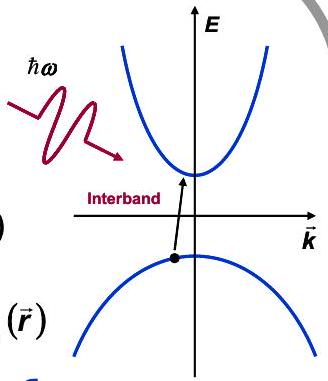
\includegraphics[alt={},max width=\textwidth]{d3f49174-c405-454e-8341-a4302bd8c868-05_381_328_386_1327}
\end{center}
\end{figure}

$\boldsymbol{N} \boldsymbol{=}$ number of primitive cells in the crystal

ECE 407 - Spring 2009 - Farhan Rana - Cornell University

\section*{Crystal Momentum Selection Rule}
$$
\begin{aligned}
& W_{\uparrow}\left(\vec{k}_{i}\right)=\frac{\mathbf{2} \pi}{\hbar}\left(\frac{e A_{o}}{\mathbf{2 m}}\right)^{\mathbf{2}} \sum_{\vec{k}_{f}}\left\langle\left\langle\psi_{c, \vec{k}_{f}}\right| e^{\left.i \vec{q} \cdot \hat{\vec{r}} \hat{\vec{P}} \cdot \hat{n}\left|\psi_{v, \vec{k}_{i}}\right\rangle\right|^{2} \delta\left(E_{c}\left(\vec{k}_{f}\right)-\right.}\right. \\
& \quad=\frac{\mathbf{2 \pi}}{\hbar}\left(\frac{e A_{o}}{\mathbf{2 m}}\right)^{\mathbf{2}} \sum_{\vec{k}_{f}}\left|\vec{P}_{c v} \cdot \hat{n}\right|^{\mathbf{2}} \delta_{\vec{k}_{i}+\vec{q}, \vec{k}_{f}} \delta\left(E_{c}\left(\vec{k}_{f}\right)-E_{v}\left(\vec{k}_{i}\right)-\hbar \omega\right) \\
& \quad=\frac{\mathbf{2 \pi}}{\hbar}\left(\frac{e A_{o}}{\mathbf{2 m}}\right)^{\mathbf{2}}\left|\vec{P}_{c v} \cdot \hat{n}\right|^{\mathbf{2}} \delta\left(E_{c}\left(\vec{k}_{i}+\vec{q}\right)-E_{v}\left(\vec{k}_{i}\right)-\hbar \omega\right)
\end{aligned}
$$

Crystal Momentum Selection Rule:\\
We have the crystal momentum selection rule:

$$
\vec{k}_{f}=\vec{k}_{i}+\vec{q}
$$

The wave vector of the photons is very small since the speed of light is very large

Therefore, one may assume that:\\
□\\
$\overrightarrow{\boldsymbol{k}}_{\boldsymbol{f}} \approx \overrightarrow{\boldsymbol{k}}_{\boldsymbol{i}}$\\
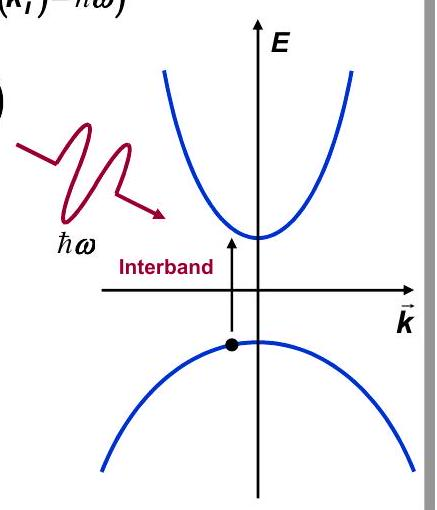
\includegraphics[max width=\textwidth, alt={}, center]{d3f49174-c405-454e-8341-a4302bd8c868-05_510_437_1766_1237}\\
$\_\_\_\_$ Optical transitions are vertical in k-space

$$
W_{\uparrow}\left(\vec{k}_{i}\right)=\frac{\mathbf{2 \pi}}{\hbar}\left(\frac{\mathbf{e} A_{o}}{\mathbf{2 m}}\right)^{\mathbf{2}}\left|\vec{P}_{c v} \cdot \hat{n}\right|^{\mathbf{2}} \delta\left(E_{c}\left(\vec{k}_{i}\right)-E_{v}\left(\vec{k}_{i}\right)-\hbar \omega\right)
$$

Generally one is not interested in the transition rate for any one particular initial electron state but in the number of transitions happening per unit volume of the material per second

The upward transition $R_{\uparrow}$ rate per unit volume is obtained by summing over all the possible initial states per unit volume weighed by the occupation probability of the initial state and\\
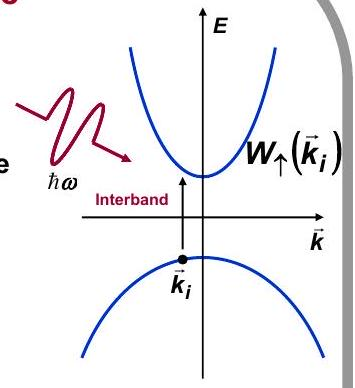
\includegraphics[max width=\textwidth, alt={}]{d3f49174-c405-454e-8341-a4302bd8c868-06_388_355_395_1319} by the probability that the final state is empty:

$$
R_{\uparrow}(\omega)=\frac{2}{V} \times \sum_{\vec{k}_{i}} W_{\uparrow}\left(\vec{k}_{i}\right) f_{v}\left(\vec{k}_{i}\right)\left[1-f_{c}\left(\vec{k}_{i}\right)\right]
$$

If we assume, as in an intrinsic semiconductor, that the valence band is full and the conduction band is empty of electrons, then:

$$
\begin{aligned}
R_{\uparrow}(\omega) & =\frac{\mathbf{2}}{V} \times \sum_{\vec{k}_{i}} W_{\uparrow}\left(\vec{k}_{i}\right) \\
& =\frac{\mathbf{2}}{V} \times \sum_{\vec{k}_{i}} \frac{\mathbf{2} \pi}{\hbar}\left(\frac{e A_{o}}{\mathbf{2 m}}\right)^{\mathbf{2}}\left|\vec{P}_{c v} \cdot \hat{n}\right|^{\mathbf{2}} \delta\left(E_{c}\left(\vec{k}_{i}\right)-E_{v}\left(\vec{k}_{i}\right)-\hbar \omega\right)
\end{aligned}
$$

\begin{center}
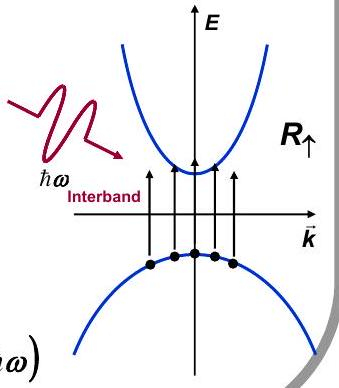
\includegraphics[max width=\textwidth, alt={}]{d3f49174-c405-454e-8341-a4302bd8c868-06_388_339_794_1327}
\end{center}

ECE 407 - Spring 2009 - Farhan Rana - Cornell University

$$
\begin{aligned}
R_{\uparrow}(\omega) & =\frac{2}{V} \times \sum_{\vec{k}_{i}} \frac{2 \pi}{\hbar}\left(\frac{e A_{o}}{2 m}\right)^{2}\left|\vec{P}_{c v} \cdot \hat{n}\right|^{2} \delta\left(E_{c}\left(\vec{k}_{i}\right)-E_{v}\left(\vec{k}_{i}\right)-\hbar \omega\right) \\
& =2 \times \int_{\mathrm{FBZ}} \frac{d^{3} \vec{k}_{i}}{(2 \pi)^{3}} \frac{2 \pi}{\hbar}\left(\frac{e A_{o}}{2 m}\right)^{2}\left|\vec{P}_{c v} \cdot \hat{n}\right|^{2} \delta\left(E_{c}\left(\vec{k}_{i}\right)-E_{v}\left(\vec{k}_{i}\right)-\hbar \omega\right) \\
& \left.=\left.\frac{2 \pi}{\hbar}\left(\frac{e A_{o}}{2 m}\right)^{2}\langle | \vec{P}_{c v} \cdot \hat{n}\right|^{2}\right\rangle \begin{array}{l}
2 \times \int_{\mathrm{FBZ}} \frac{d^{3} \vec{k}_{i}}{(2 \pi)^{3}} \delta\left(E_{c}\left(\vec{k}_{i}\right)-E_{v}\left(\vec{k}_{i}\right)-\hbar \omega\right) \\
\left.2 \times\left.\left(\frac{e A_{o}}{2 m}\right)^{2}\langle | \vec{P}_{c v} \cdot \hat{n}\right|^{2}\right\rangle \underbrace{2 \times \int_{\mathrm{FBZ}} \frac{d^{3} \vec{k}}{(2 \pi)^{3}} \delta\left(E_{c}(\vec{k})-E_{v}(\vec{k})-\hbar \omega\right)}_{\text {Joint density of states }}
\end{array} \\
= & \frac{2 \pi}{\hbar} \underbrace{2 \pi}\left(\frac{e}{2 \pi}\right)
\end{aligned}
$$

\begin{figure}[h]
\begin{center}
\captionsetup{labelformat=empty}
\caption{Transition Rates per Unit Volume}
  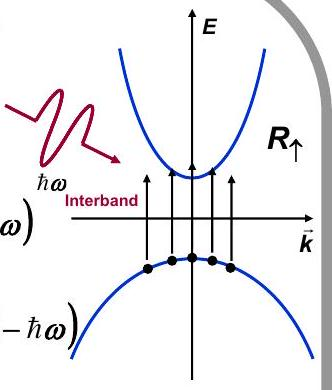
\includegraphics[alt={},max width=\textwidth]{d3f49174-c405-454e-8341-a4302bd8c868-06_390_332_1559_1340}
\end{center}
\end{figure}

The integral in the expression above is similar to the density of states integral:\\
Suppose: $E_{c}(\overrightarrow{\boldsymbol{k}})=E_{c}+\frac{\hbar^{2} \boldsymbol{k}^{2}}{\mathbf{2} \boldsymbol{m}_{e}}$\\
Then: $\quad g_{3 D}(E)=2 \times \int_{\mathrm{FBZ}} \frac{d^{3} \vec{k}}{(2 \pi)^{3}} \delta\left(E_{c}(\vec{k})-E\right)=\frac{1}{2 \pi^{2}}\left(\frac{2 m_{e}}{\hbar^{2}}\right)^{3 / 2} \sqrt{E-E_{c}}$

\section*{Transition Rates per Unit Volume and Joint Density of States}
$$
\left.R_{\uparrow}(\omega)=\left.\frac{2 \pi}{\hbar}\left(\frac{e A_{o}}{2 m}\right)^{2}\langle | \vec{P}_{c v} \cdot \hat{n}\right|^{2}\right\rangle 2 \times \int_{\mathrm{FBZ}} \frac{d^{3} \vec{k}}{(2 \pi)^{3}} \delta\left(E_{c}(\vec{k})-E_{v}(\vec{k})-\hbar \omega\right)
$$

Suppose: $\quad E_{c}(\vec{k})=E_{c}+\frac{\hbar^{2} k^{2}}{\mathbf{2} \boldsymbol{m}_{e}} \quad E_{v}(\overrightarrow{\boldsymbol{k}})=E_{v}-\frac{\hbar^{2} \boldsymbol{k}^{2}}{\mathbf{2} \boldsymbol{m}_{\boldsymbol{h}}}$

Reduced effective mass

Then :

$$
E_{c}(\vec{k})-E_{v}(\vec{k})=E_{c}-E_{v}+\frac{\hbar^{2} k^{2}}{2}\left(\frac{1}{m_{e}}+\frac{1}{m_{h}}\right)=E_{g}+\frac{\hbar^{2} k^{2}}{2 m_{r}}
$$

$$
\left.R_{\uparrow}(\omega)=\left.\frac{2 \pi}{\hbar}\left(\frac{e A_{o}}{2 m}\right)^{2}\langle | \vec{P}_{c v} \cdot \hat{n}\right|^{2}\right\rangle \frac{1}{2 \pi^{2}}\left(\frac{2 m_{r}}{\hbar^{2}}\right)^{3 / 2} \sqrt{\hbar \omega-E_{g}}
$$

\begin{center}
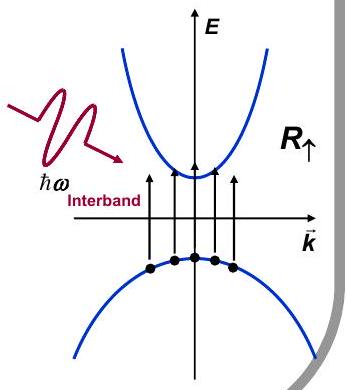
\includegraphics[max width=\textwidth, alt={}]{d3f49174-c405-454e-8341-a4302bd8c868-07_390_347_790_1327}
\end{center}

ECE 407 - Spring 2009 - Farhan Rana - Cornell University

\section*{Transition Rates per Unit Volume}
$\left.\boldsymbol{R}_{\uparrow}(\omega)=\left.\frac{\mathbf{2} \boldsymbol{\pi}}{\hbar}\left(\frac{\mathbf{e} A_{o}}{\mathbf{2} \boldsymbol{m}}\right)^{\mathbf{2}}\langle | \vec{P}_{c v} \cdot \hat{\boldsymbol{n}}\right|^{\mathbf{2}}\right\rangle \frac{\mathbf{1}}{\mathbf{2} \boldsymbol{\pi}^{\mathbf{2}}}\left(\frac{\mathbf{2} \boldsymbol{m}_{r}}{\hbar^{\mathbf{2}}}\right)^{\mathbf{3} / \mathbf{2}} \sqrt{\hbar \omega-E_{g}}$\\
The power per unit area or the Intensity of the E\&M wave is:

$$
I=\frac{\omega^{2} A_{\mathrm{o}}^{2}}{2 \eta}
$$

$\left.R_{\uparrow}(\omega)=\left.\frac{\mathbf{2} \boldsymbol{\pi}}{\hbar}\left(\frac{\mathbf{e}}{\mathbf{2} \boldsymbol{m}}\right)^{\mathbf{2}}\left(\frac{\mathbf{2} \eta I}{\boldsymbol{\omega}^{\mathbf{2}}}\right)\langle | \vec{P}_{c v} \cdot \hat{\boldsymbol{n}}\right|^{\mathbf{2}}\right\rangle \frac{\mathbf{1}}{\mathbf{2} \boldsymbol{\pi}^{\mathbf{2}}}\left(\frac{\mathbf{2} \boldsymbol{m}_{r}}{\hbar^{\mathbf{2}}}\right)^{\mathbf{3} / \mathbf{2}} \sqrt{\hbar \omega-E_{g}}$\\
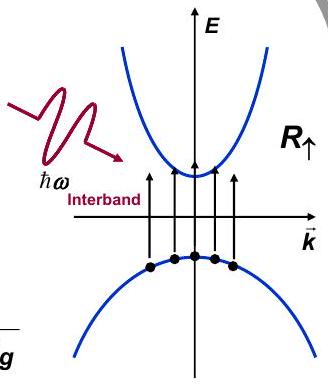
\includegraphics[max width=\textwidth, alt={}, center]{d3f49174-c405-454e-8341-a4302bd8c868-07_388_328_1602_1327}

Interband Momentum Matrix Elements:\\
Recall the result from homework 7:

$$
\frac{1}{m_{r}}=\left(\frac{1}{m_{e}}+\frac{1}{m_{h}}\right)=\frac{4}{m^{2}} \frac{\left|\vec{P}_{c v} \cdot \hat{n}\right|^{2}}{E_{g}}
$$

The above result assumed diagonal isotropic conduction and valence bands and also that no other bands are present, and is therefore oversimplified\\
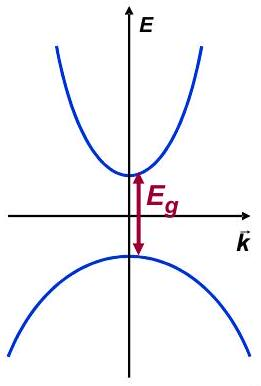
\includegraphics[max width=\textwidth, alt={}, center]{d3f49174-c405-454e-8341-a4302bd8c868-07_386_261_2023_1284}

\section*{Momentum Matrix Elements}
In bulk III-V semiconductors with cubic symmetry, the average value of the momentum matrix element is usually expressed in terms of the energy $E_{p}$ as,

$$
\left.\left.\langle | \vec{P}_{c v} \cdot \hat{n}\right|^{2}\right\rangle=\frac{m E_{p}}{6}
$$

Note that the momentum matrix elements are independent of the direction of light polarization!

\begin{center}
\begin{tabular}{|l|r|r|r|r|r|}
\hline
Parameters at 300K & GaAs & \multicolumn{1}{|c|}{AlAs} & \multicolumn{1}{c|}{InAs} & \multicolumn{1}{c|}{InP} & \multicolumn{1}{c|}{GaP} \\
\hline
Ep (eV) & 25.7 & 21.1 & 22.2 & 20.7 & 22.2 \\
\hline
\end{tabular}
\end{center}

\section*{Transition Rates per Unit Volume and the Absorption or Loss Coefficient}
Because of transitions photons will be lost from the E\&M wave traveling inside the solid. This loss will result in decay of the wave Intensity with distance travelled:

$$
\begin{aligned}
& \Rightarrow I(x)=\mathrm{e}^{-\alpha x} I(x=0) \\
& \Rightarrow \frac{I(x)}{d x}=-\alpha I(x) \\
& \Rightarrow I(x+\Delta x)-I(x)=-\alpha \Delta x I(x)
\end{aligned}
$$

\begin{center}
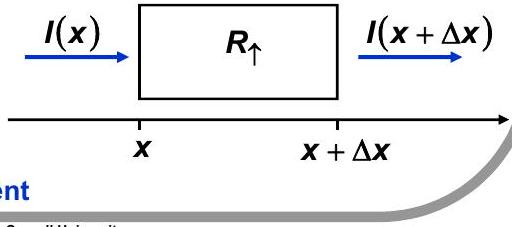
\includegraphics[max width=\textwidth, alt={}]{d3f49174-c405-454e-8341-a4302bd8c868-08_227_512_1005_1138}
\end{center}

Loss coefficient or absorption coefficient

\section*{Transition Rates per Unit Volume and Loss Coefficient}
$\Rightarrow I(x+\Delta x)-I(x)=-\alpha \quad \Delta x I(x)$\\
The wave power loss (per unit area) in small distance $\boldsymbol{\Delta x}$ is $\boldsymbol{\alpha} \boldsymbol{\Delta} \boldsymbol{x} \boldsymbol{I} \boldsymbol{(} \boldsymbol{x} \boldsymbol{)}$\\
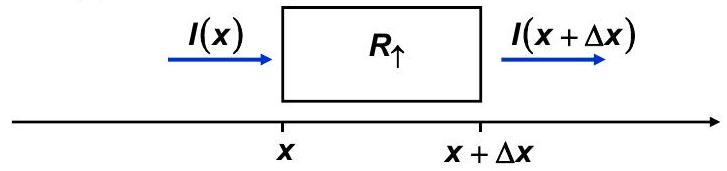
\includegraphics[max width=\textwidth, alt={}, center]{d3f49174-c405-454e-8341-a4302bd8c868-08_171_727_1757_509}

The wave power loss in small distance $\Delta x$ must also equal: $\hbar \omega R_{\uparrow} \Delta x$\\
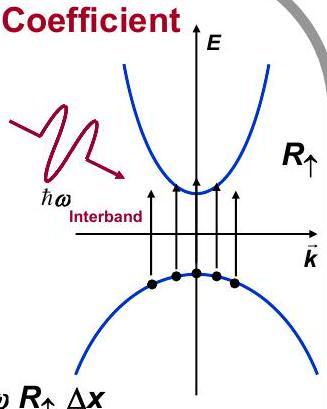
\includegraphics[max width=\textwidth, alt={}, center]{d3f49174-c405-454e-8341-a4302bd8c868-08_409_327_1564_1334}

Therefore:

$$
\begin{aligned}
& \hbar \omega R_{\uparrow} \Delta x=\alpha \Delta x I \\
& \begin{aligned}
\Rightarrow \alpha(\omega)=\frac{\hbar \omega R_{\uparrow}(\omega)}{I} & =2 \pi\left(\frac{e}{2 m}\right)^{2}\left(\frac{2 \eta}{\omega}\right)\left|\vec{P}_{c V} \cdot \hat{n}\right|^{2} \frac{1}{2 \pi^{2}}\left(\frac{2 m}{\hbar^{2}}\right)^{3 / 2} \sqrt{\hbar \omega-E_{g}} \\
& =\left(\frac{e}{m}\right)^{2} \frac{\pi}{\varepsilon_{o} n \omega c}\left|\vec{P}_{c V} \cdot \hat{n}\right|^{2} \frac{1}{2 \pi^{2}}\left(\frac{2 m}{\hbar^{2}}\right)^{3 / 2} \sqrt{\hbar \omega-E_{g}}
\end{aligned}
\end{aligned}
$$

Values of $\boldsymbol{\alpha}(\boldsymbol{\omega})$ for most semiconductors can range from a few hundred $\mathbf{c m}^{\boldsymbol{-} \mathbf{1}}$ to hundred thousand $\mathbf{c m}^{\boldsymbol{-} \mathbf{1}}$\\
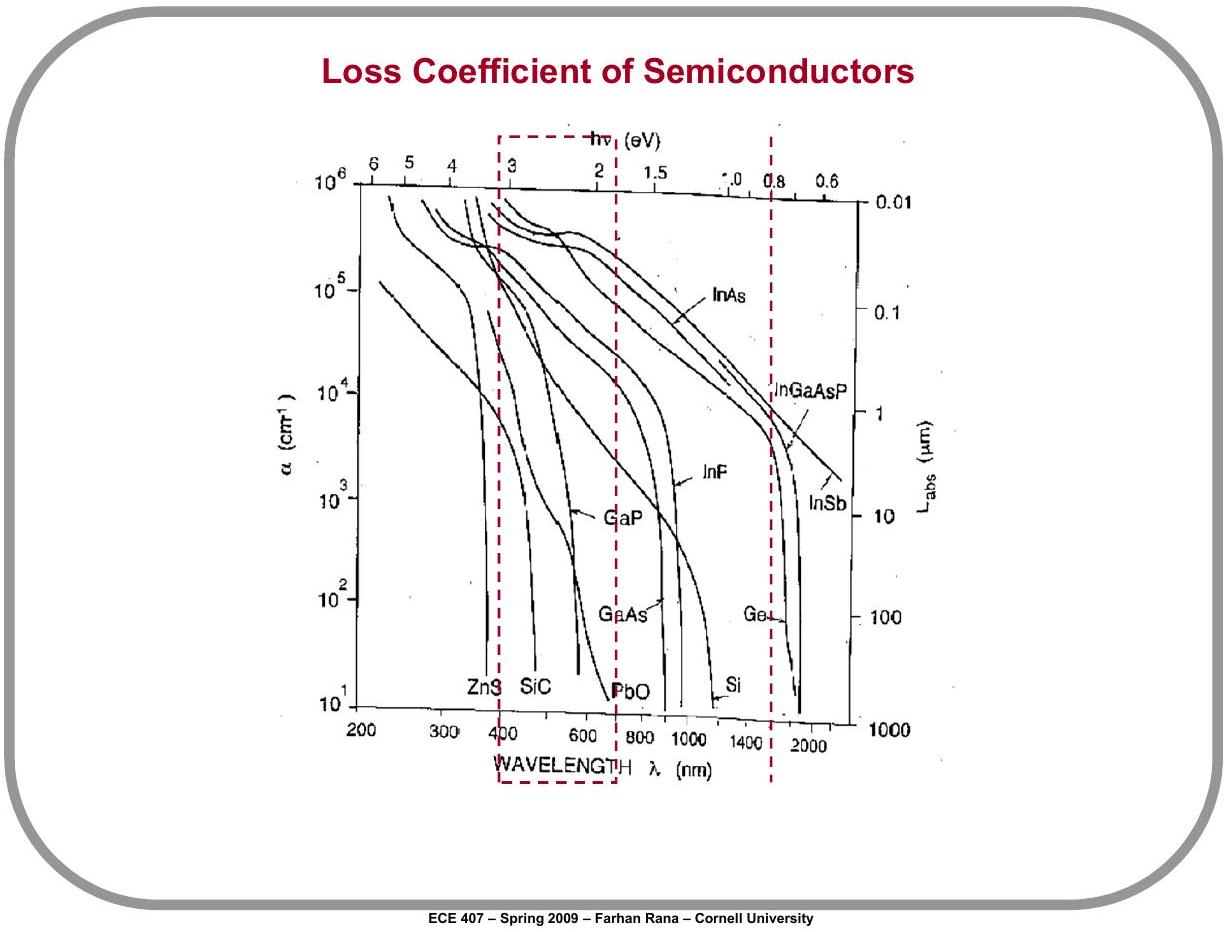
\includegraphics[max width=\textwidth, alt={}, center]{d3f49174-c405-454e-8341-a4302bd8c868-09_932_1229_317_449}\\
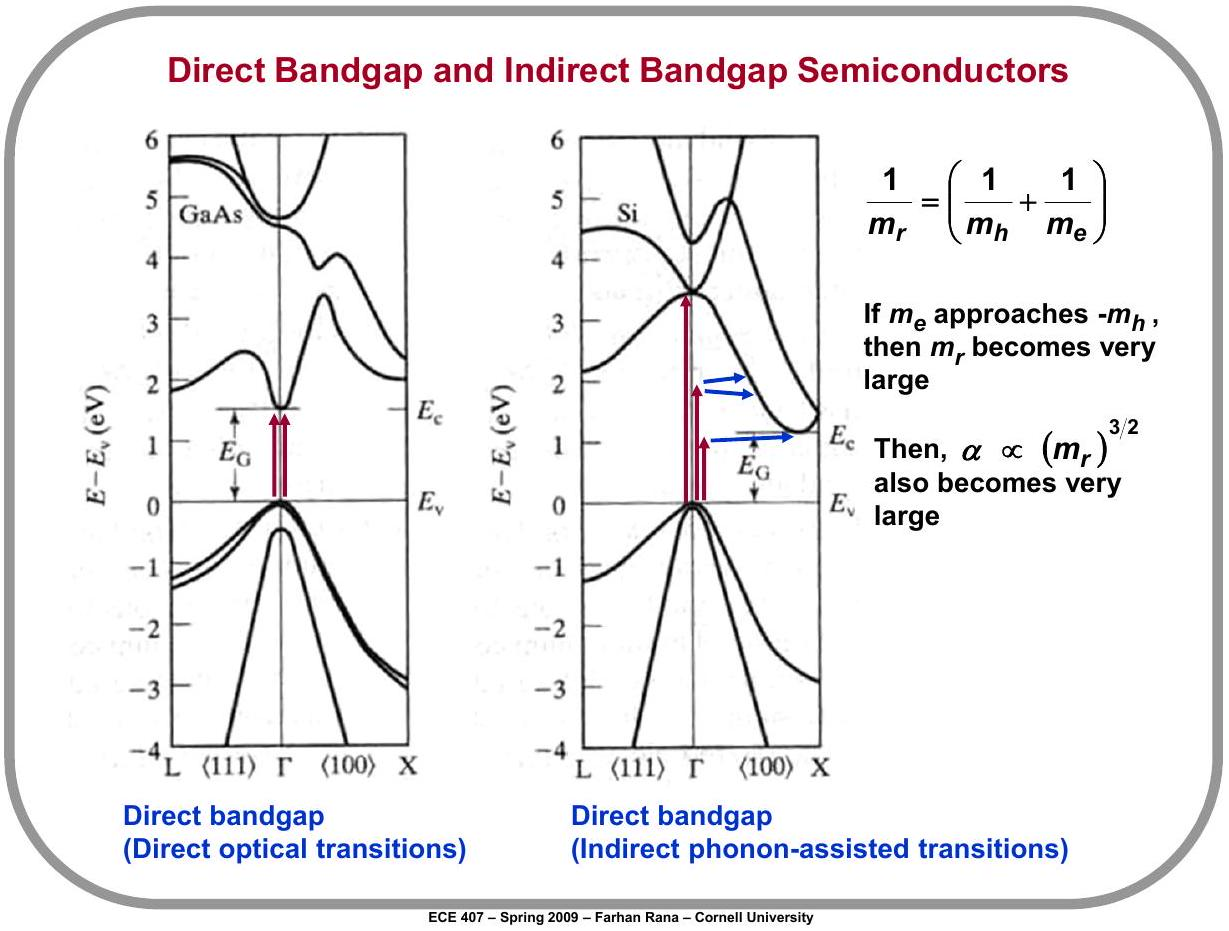
\includegraphics[max width=\textwidth, alt={}, center]{d3f49174-c405-454e-8341-a4302bd8c868-09_931_1229_1514_449}

\section*{Stimulated Absorption and Stimulated Emission}
Throwing back in the occupation factors one can write more generally:

$$
\left.R_{\uparrow}(\omega)=\left.\frac{2 \pi}{\hbar}\left(\frac{e A_{o}}{2 m}\right)^{2}\langle | \vec{P}_{c v} \cdot \hat{n}\right|^{2}\right\rangle 2 \times \int_{\mathrm{FBZ}} \frac{d^{3} \vec{k}}{(2 \pi)^{3}} f_{v}(\vec{k})\left[1-f_{c}(\vec{k})\right] \delta\left(E_{c}(\vec{k})-E_{v}(\vec{k})-\hbar \omega\right)
$$

\section*{Stimulated Absorption:}
The process of photon absorption is called stimulated absorption (because, quite obviously, the process is initiated by the incoming radiation or photons some of which eventually end up getting absorbed)\\
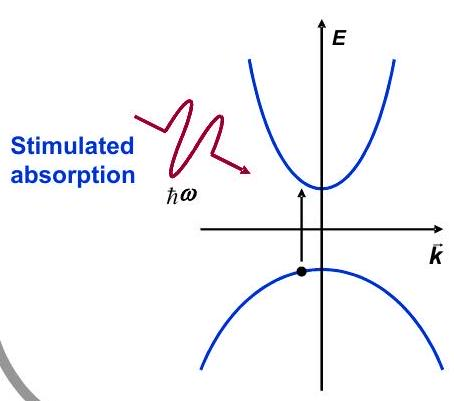
\includegraphics[max width=\textwidth, alt={}, center]{d3f49174-c405-454e-8341-a4302bd8c868-10_401_454_779_471}

An incoming photon can also cause the reverse process in which an electron makes a downward transition

This reverse process is initiated by the term in Hamiltonian that has the $\boldsymbol{e}^{i \omega t}$ time dependence:

$$
\begin{gathered}
\hat{H}=\hat{H}_{o}+\hat{V}_{\uparrow} \mathrm{e}^{-i \omega t}+\hat{V}_{\downarrow} \mathrm{e}^{i \omega t} \\
\hat{V}_{\uparrow}=\frac{e A_{o} \mathrm{e}^{i \bar{q}} \cdot \hat{\vec{r}}}{2 m} \hat{\vec{P}} \cdot \hat{n} \quad \hat{V}_{\downarrow}=\frac{e A_{o} \mathrm{e}^{-i \vec{q} \cdot \hat{r}}}{2 m} \hat{\vec{P}} \cdot \hat{n}
\end{gathered}
$$

ECE 407 - Spring 2009 - Farhan Rana - Cornell University

\section*{Stimulated Emission and Spontaneous Emission}
Following the same procedure as for stimulated absorption, one can write the rate per unit volume for the downward transitions as:

$$
\left.R_{\downarrow}(\omega)=\left.\frac{2 \pi}{\hbar}\left(\frac{e A_{o}}{2 m}\right)^{2}\langle | \vec{P}_{c v} \cdot \hat{n}\right|^{2}\right\rangle 2 \times \int_{\mathrm{FBZ}} \frac{d^{3} \vec{k}}{(2 \pi)^{3}} f_{c}(\vec{k})\left[1-f_{v}(\vec{k})\right] \delta\left(E_{c}(\vec{k})-E_{v}(\vec{k})-\hbar \omega\right)
$$

Stimulated Emission:\\
In the downward transition, the electron gives off its energy to the electromagnetic field, i.e. it emits a photon! The process of photon emission caused by incoming radiation (or by other photons) is called stimulated emission.

Spontaneous Emission:\\
Electrons can also make downward transitions even in the absence of any incoming radiation (or photons). This process is called spontaneous emission.\\
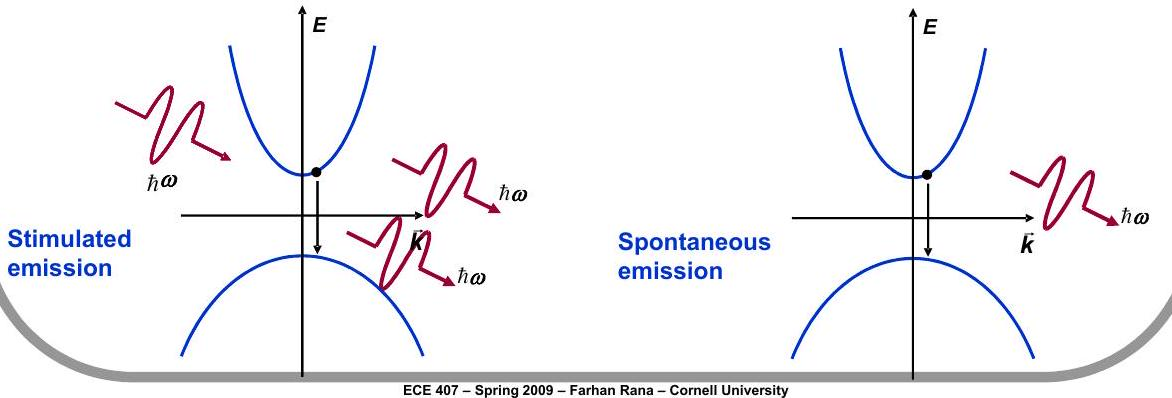
\includegraphics[max width=\textwidth, alt={}, center]{d3f49174-c405-454e-8341-a4302bd8c868-10_398_1172_2041_474}

\section*{Stimulated Absorption and Stimulated Emission}
The net stimulated electronic transition rate is the difference between the stimulated emission and stmulated absorption rates:

$$
\left.R_{\uparrow}(\omega)-R_{\downarrow}(\omega)=\left.\frac{2 \pi}{\hbar}\left(\frac{e A_{o}}{2 m}\right)^{2}\langle | \vec{P}_{c v} \cdot \hat{n}\right|^{2}\right\rangle 2 \times \int_{\mathrm{FBZ}} \frac{d^{3} \vec{k}}{(2 \pi)^{3}}\left[f_{v}(\vec{k})-f_{c}(\vec{k})\right] \delta\left(E_{c}(\vec{k})-E_{v}(\vec{k})-\hbar \omega\right)
$$

And the more accurate expression for the loss coefficient is then:

$$
\begin{aligned}
\alpha(\omega) & =\frac{\hbar \omega\left(R_{\uparrow}(\omega)-R_{\downarrow}(\omega)\right)}{I} \\
& \left.=\left.\left(\frac{\mathbf{e}}{m}\right)^{2} \frac{\pi}{\varepsilon_{0} n \omega c}\langle | \vec{P}_{c v} \cdot \hat{n}\right|^{2}\right\rangle 2 \times \int_{\mathrm{FBZ}} \frac{d^{3} \vec{k}}{(2 \pi)^{3}}\left[f_{v}(\vec{k})-f_{c}(\vec{k})\right] \delta\left(E_{c}(\vec{k})-E_{v}(\vec{k})-\hbar \omega\right)
\end{aligned}
$$

\begin{center}
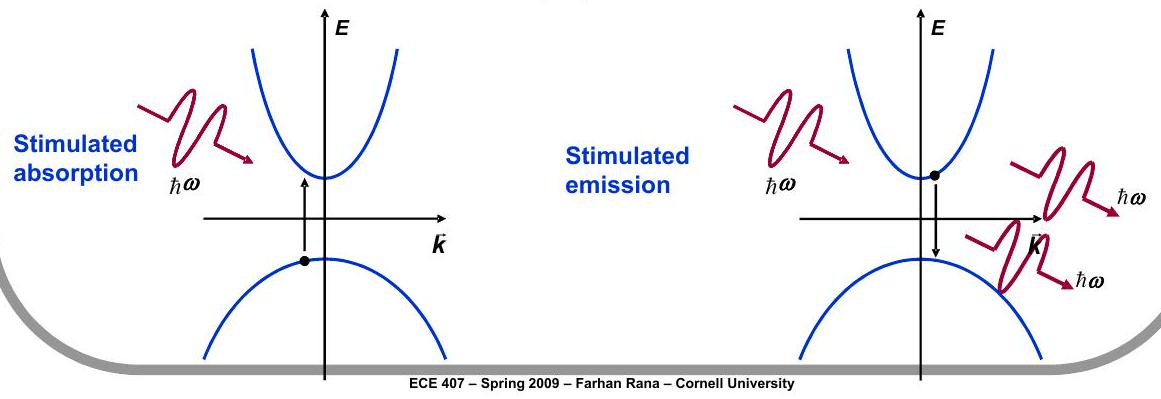
\includegraphics[max width=\textwidth, alt={}]{d3f49174-c405-454e-8341-a4302bd8c868-11_399_1161_852_468}
\end{center}

\section*{Optical Gain in Semiconductors}
$$
\left.\alpha(\omega)=\left.\left(\frac{e}{m}\right)^{2} \frac{\pi}{\varepsilon_{0} n \omega c}\langle | \vec{P}_{c v} \cdot \hat{n}\right|^{2}\right\rangle 2 \times \int_{\mathrm{FBZ}} \frac{d^{3} \vec{k}}{(2 \pi)^{3}}\left[f_{v}(\vec{k})-f_{c}(\vec{k})\right] \delta\left(E_{c}(\vec{k})-E_{v}(\vec{k})-\hbar \omega\right)
$$

Note that the Intensity decays as: $I(x)=e^{-\alpha x} I(x=0)$

What if $\alpha$ were to become negative? Optical gain !!

$$
\alpha(\omega)<0 \Rightarrow R_{\downarrow}(\omega)>R_{\uparrow}(\omega)
$$

A negative value of $\alpha$ implies optical gain (as opposed to optical loss) and means that stimulated emission rate exceeds stimulated absorption rate

\section*{Optical gain is possible if:}
\begin{center}
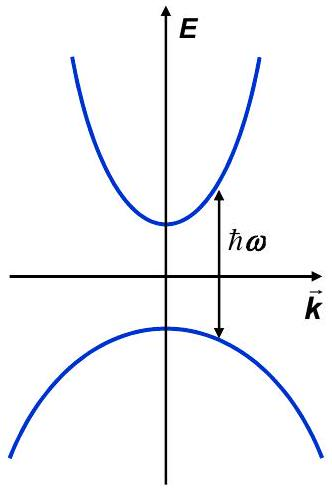
\includegraphics[max width=\textwidth, alt={}]{d3f49174-c405-454e-8341-a4302bd8c868-11_490_332_1738_1306}
\end{center}

$$
\begin{aligned}
& f_{v}(\vec{k})-f_{c}(\vec{k})<0 \quad \text { for } \quad \\
& \Rightarrow f_{c}(\vec{k})-f_{v}(\vec{k})>0 \quad \text { for } \quad E_{c}(\vec{k})-E_{v}(\vec{k})=\hbar \omega \\
& \quad E_{v}(\vec{k})-E_{v}(\vec{k})=\hbar \omega
\end{aligned}
$$

\section*{Optical Gain in Semiconductors}
Optical gain is only possible in non-equilibrium situations when the electron and hole Fermi levels are not the same

Suppose:

$$
\begin{aligned}
& f_{c}(\vec{k})=f\left(E_{c}(\vec{k})-E_{f e}\right)=\frac{1}{1+e^{\left(E_{c}(\vec{k})-E_{f e}\right) / K T}} \\
& f_{v}(\vec{k})=f\left(E_{v}(\vec{k})-E_{f h}\right)=\frac{1}{1+e^{\left(E_{v}(\vec{k})-E_{f h}\right) / K T}} \\
& E_{c}(\vec{k})-E_{v}(\vec{k})=\hbar \omega
\end{aligned}
$$

Then the condition for optical gain at frequency $\omega$ is:

$$
\begin{aligned}
& f\left(E_{c}(\vec{k})-E_{f e}\right)-f\left(E_{v}(\vec{k})-E_{f h}\right)>0 \\
& \Rightarrow E_{f e}-E_{f h}>E_{c}(\vec{k})-E_{v}(\vec{k}) \\
& \Rightarrow E_{f e}-E_{f h}>\hbar \omega
\end{aligned}
$$

\begin{center}
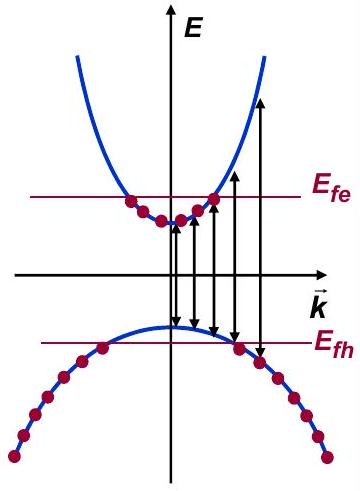
\includegraphics[max width=\textwidth, alt={}]{d3f49174-c405-454e-8341-a4302bd8c868-12_491_360_543_1301}
\end{center}

The above is the condition for population inversion (lots of electrons in the conduction band and lots of holes in the valence band)

ECE 407 - Spring 2009 - Farhan Rana - Cornell University

\section*{Optical Gain in Semiconductors}
The loss coefficient is a function of frequency:

$$
\left.\alpha(\omega)=\left.\left(\frac{e}{m}\right)^{2} \frac{\pi}{\varepsilon_{0} n \omega c}\langle | \vec{P}_{c v} \cdot \hat{n}\right|^{2}\right\rangle 2 \times \int_{\mathrm{FBZ}} \frac{d^{3} \vec{k}}{(2 \pi)^{3}}\left[f_{v}(\vec{k})-f_{c}(\vec{k})\right] \delta\left(E_{c}(\vec{k})-E_{v}(\vec{k})-\hbar \omega\right)
$$

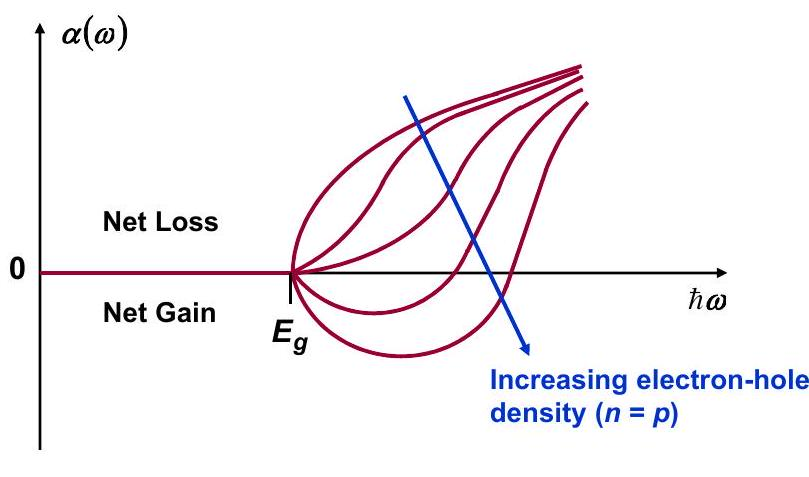
\includegraphics[max width=\textwidth, alt={}, center]{d3f49174-c405-454e-8341-a4302bd8c868-12_477_809_1804_481}\\
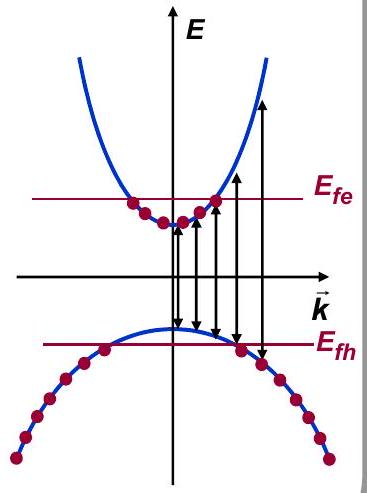
\includegraphics[max width=\textwidth, alt={}, center]{d3f49174-c405-454e-8341-a4302bd8c868-12_493_367_1800_1299}

Optical gain for frequencies for which:

$$
E_{g}<\hbar \omega<E_{f e}-E_{f h}
$$

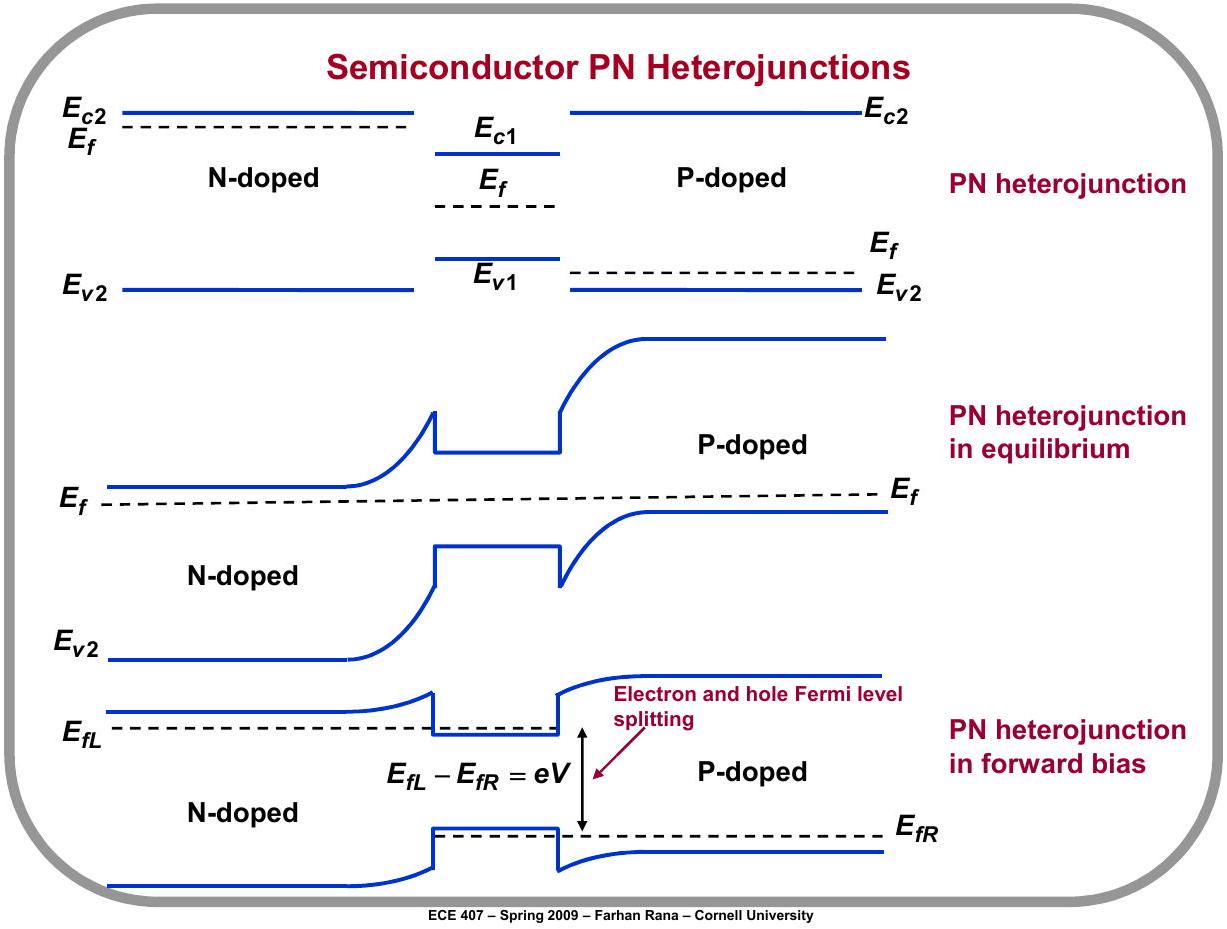
\includegraphics[max width=\textwidth, alt={}, center]{d3f49174-c405-454e-8341-a4302bd8c868-13_929_1227_320_449}\\
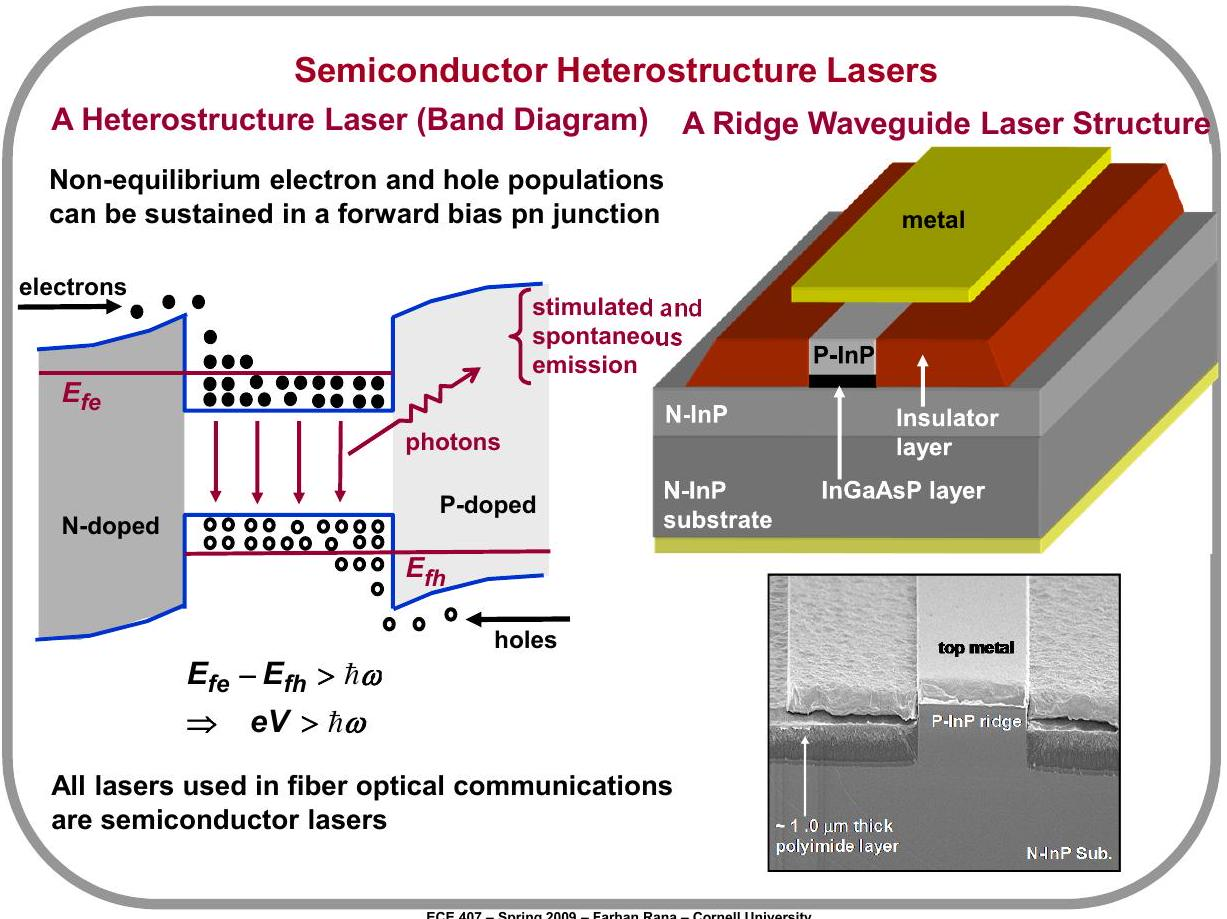
\includegraphics[max width=\textwidth, alt={}, center]{d3f49174-c405-454e-8341-a4302bd8c868-13_919_1227_1514_451}\\
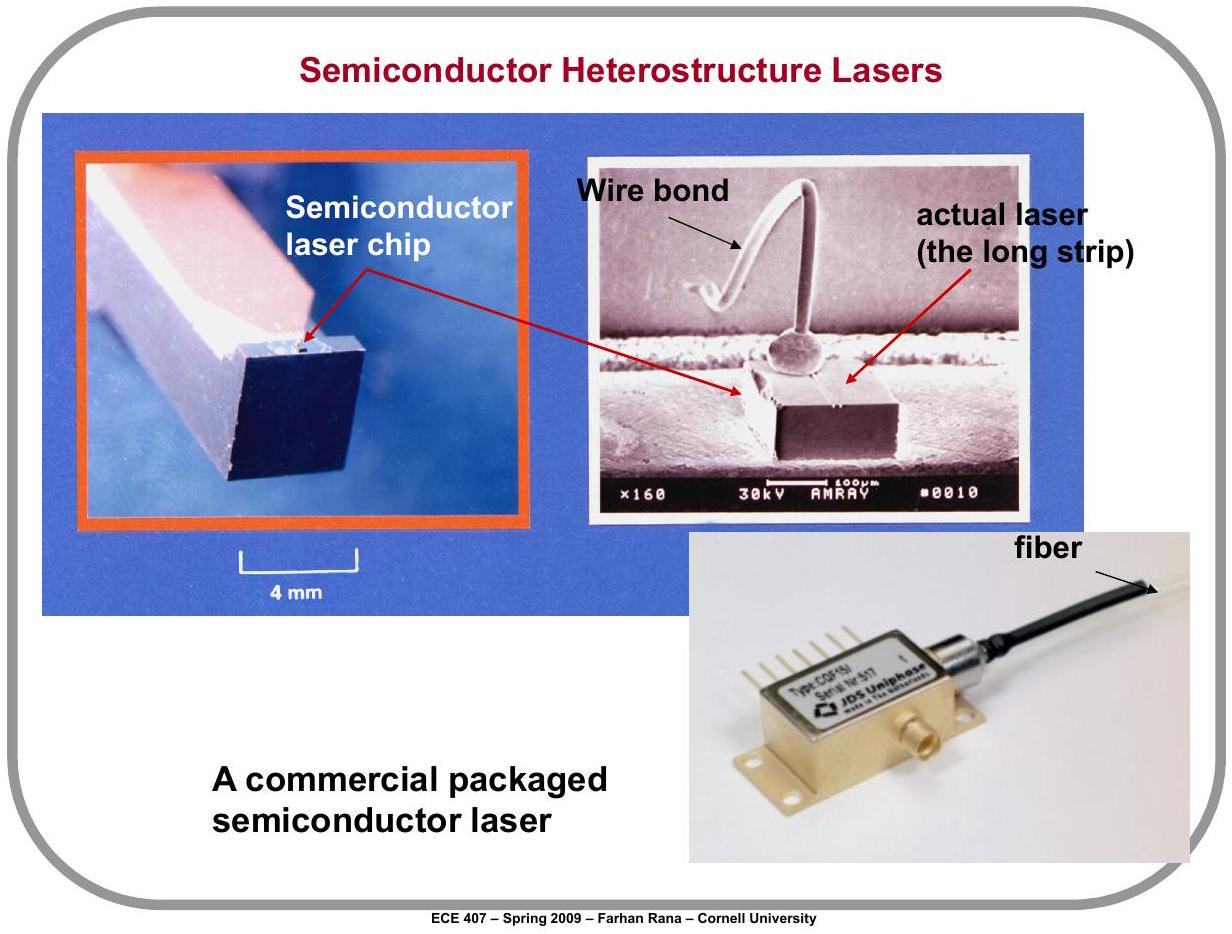
\includegraphics[max width=\textwidth, alt={}, center]{d3f49174-c405-454e-8341-a4302bd8c868-14_934_1232_317_446}


\end{document}